\documentclass[12pt, letterpaper]{book}
\usepackage{amsfonts, amsmath, amssymb, mathtools, amsthm, mathrsfs}
\usepackage{parskip}
\usepackage{xfrac}
\usepackage{tikz, tikz-3dplot}
\usepackage[most]{tcolorbox}
\usepackage{physics}
\usepackage{lmodern}
\usepackage{cleveref}
\usepackage[letterpaper, textwidth= 6in, textheight= 8.5in, headsep=.5in, voffset= 0.3in]{geometry}
\usetikzlibrary{decorations.pathreplacing,calligraphy, shapes}

\tolerance=1
\emergencystretch=\maxdimen
\hyphenpenalty=10000
\hbadness=10000

\title{Mathematical Physics Notes}
\author{Pratik T}

\begin{document}

% \maketitle

\chapter{Complex Analysis}

\section{Stereographic Projection}


Complex variables are of the form: $$z= x+ iy, \ \ (x,y\ \  \epsilon\  \mathbb{R}) $$
Here $x$ and $y$ are linearly independent variables. Moreover, the complex conjugate of $z$, $$z^*= x-iy$$ is also linearly independent of $z$.
Unlike the real number line, where we can tend to $\infty$ by going leftwards or rightwards from the origin, the complex plane is 2-dimensional. Thus, we can tend to $\infty$ in an infinite number of ways, i.e., along any ray passing through the origin. To get rid of this inconvenience, we map the entire 2D complex plane to a 3D hollow sphere. As we will see, this will allow us to treat $\infty$ just like any finite point. 

First we take the complex plane, and sew its ends together, making a unit sphere, called the Riemann sphere. If the coordinates on the sphere are $\xi_1, xi_2$ and $\xi_3$ then they will obviously satisfy the constraints: 

\begin{equation}
    \begin{aligned}
        \xi_1 &= \sin\theta\cos\phi\\
        \xi_2 &= \sin\theta\sin\phi\\
        \xi_3 &= \cos\theta 
    \end{aligned} \label{eq1}
\end{equation}

\begin{figure}
    \begin{center}
        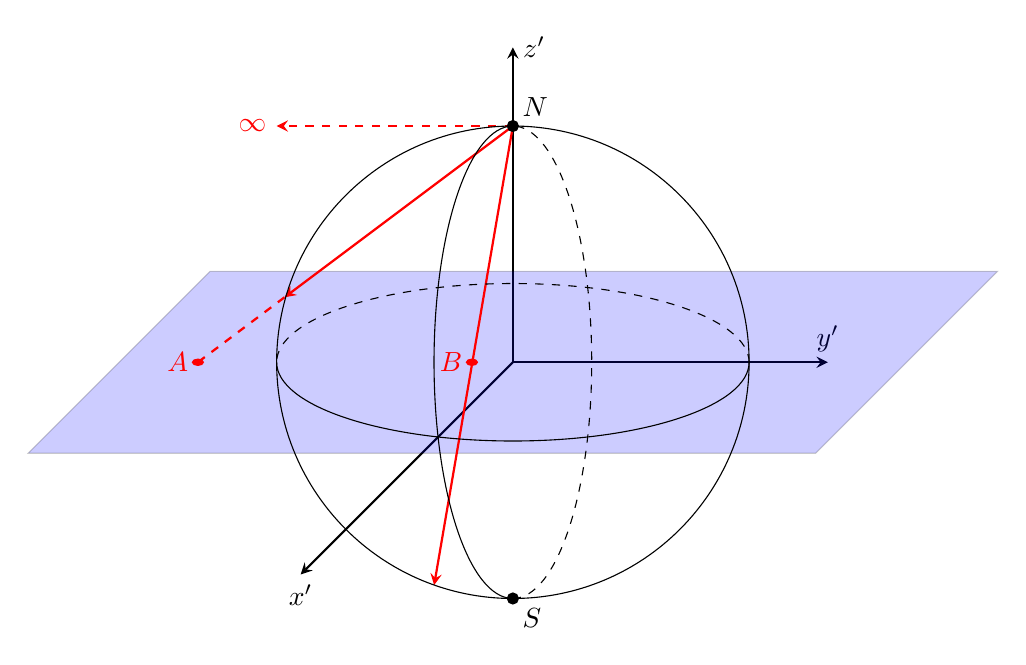
\begin{tikzpicture}

            \draw[thick,-stealth] (0,0,0)--(4,0,0) node[above]  {$y'$};
            \draw[thick,-stealth] (0,0,0)--(0,4,0) node[right]  {$z'$};
            \draw[thick,-stealth] (0,0,0)--(0,0,7) node[below]  {$x'$}; 

            \filldraw[draw=black, fill= blue, opacity= 0.2] (-5,0,  3)--(5,0,3)--(5,0,-3)--(-5,0,-3)--cycle;

            \draw[thick, -stealth, red] (0,3,0)->(-1,-2.83,0);
            \filldraw[red] (-0.52,0,0) ellipse(0.07 and 0.04) node  [left] {$B$};

            \draw[thick, -stealth, red] (0,3,0)->(-2.9,0.825,0);
            \draw[thick, dashed, red] (-2.9,0.825)--(-4,0,0);
            \filldraw[red] (-4,0,0) ellipse(0.07 and 0.04) node [left] {$A$};

            \draw[thick, dashed, -stealth, red] (0,3,0)--(-3,3,0)   node[left] {$\infty$};

            \draw(0,0,0) circle (3);
            \draw[black, dashed] (3,0,0) arc(0:180:3 and 1);
            \draw[black] (-3,0,0) arc(-180:0:3 and 1);

            \tdplotsetmaincoords{90}{90}
            \tdplotsetthetaplanecoords{-19.5}
            \tdplotdrawarc[tdplot_rotated_coords, black]{(0,0,0)}   {3}{0}{180}{anchor=south west}{}
            \tdplotsetthetaplanecoords{-19.5}
            \tdplotdrawarc[tdplot_rotated_coords, black, dashed]    {(0,0,0)}{3}{180}{360}{anchor=south west}{}

            \filldraw [black] (0,3,0) circle(0.07) node[anchor= south west] {$N$};
            \filldraw [black] (0,-3,0) circle(0.07) node[anchor= north west] {$S$};

        \end{tikzpicture}
        \caption{\emph{Stereographic Projection from the complex plane to a hollow unit sphere}}
        \label{stereo}    
    \end{center}
\end{figure}

In \cref{stereo}, the blue sheet represents the complex plane, while the sphere is the Riemann sphere. The mapping is done as follows: start from the north pole and spread out rays from this point. Anytime the ray intersects the complex plane, trace that ray back to see where it intersects the sphere. The point of intersection is the mapped coordinate. It can be seen that all points (like $A$) which lie oustide the circular plane of intersection of the complex plane and the Riemann sphere, are mapped to the northern hemisphere. The points which lie inside this circular plane (like $B$) are mapped to the southern hemisphere. Then $\infty$ gets mapped to a single point which is the north pole, as required. The origin gets mapped to the south pole. The equator of the sphere is the unit circle in the complex plane, where $|z|= 1$.

We now look for coordinate transformations which link the coordinates on the sphere to those in the complex plane. Consider the $x'-z'$ plane. 

\begin{figure}
    \begin{center}
        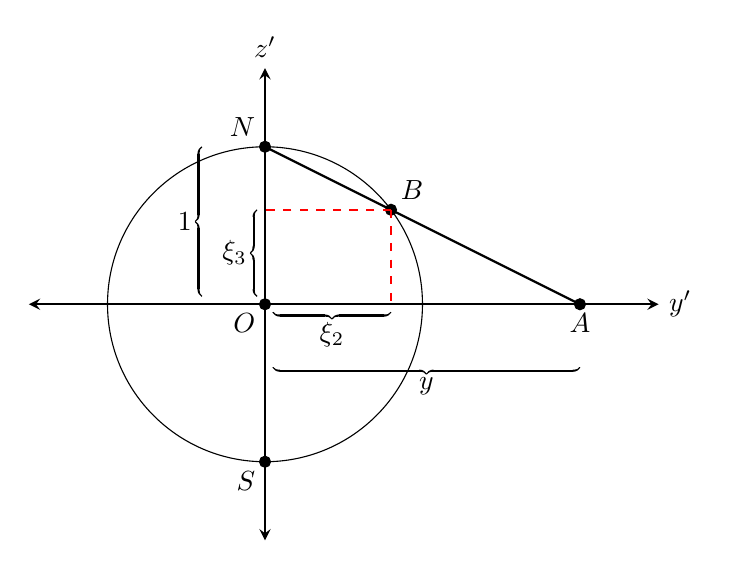
\begin{tikzpicture}

            \draw(0,0) circle (2);
            \draw[thick,stealth-stealth] (-3,0)--(5,0) node[right] {$y'$};
            \draw[thick,stealth-stealth] (0,-3)--(0,3) node[above] {$z'$};

            \filldraw [black] (0,2) circle(0.07) node[anchor= south east] {$N$};
            \filldraw [black] (0,0) circle(0.07) node[anchor= north east] {$O$};
            \filldraw [black] (0,-2) circle(0.07) node[anchor= north east] {$S$};
            \filldraw [black] (1.6, 1.2) circle(0.07) node[anchor= south west] {$B$};
            \filldraw [black] (4, 0) circle(0.07) node[below] {$A$};

            \draw[thick, black] (0,2)--(4,0);
            \draw[thick, dashed, red] (1.6, 1.2)--(1.6,0);
            \draw[thick, dashed, red] (1.6, 1.2)--(0,1.2);

            \draw [thick, decorate, decoration = {calligraphic brace, mirror}] (-0.1, 1.2)--(-0.1,0.1) node[ pos= 0.5, left] {$\xi_3$};
            \draw [thick, decorate, decoration = {calligraphic brace,mirror}] (0.1,-0.1)--(1.6, -0.1) node[ pos= 0.5, below] {$\xi_2$};
            \draw [thick, decorate, decoration = {calligraphic brace, mirror}] (-0.8, 2)--(-0.8,0.1) node[ pos= 0.5, left] {$1$};
            \draw [thick, decorate, decoration = {calligraphic brace, mirror}] (0.1,-0.8)--(4, -0.8) node[ pos= 0.5, below] {$y$};

        \end{tikzpicture}
        \caption{\emph{Stereographic Progection in the $y'-z'$ plane. Point $A$ in the complex plane is purely imaginary since it lies on the $y'$ axis ($z= x'+iy'$). It is mapped to point $B$ on the Riemann sphere.}}
        \label{stereo2}    
    \end{center}
\end{figure}

Since the upper triangle and the big triangle are similar in Figure \cref{stereo2}, by property of similar triangles we have
    $$\frac{\xi_2}{y}= \frac{1-\xi_3}{1}$$
    \begin{equation} y= \frac{\xi_2}{1-\xi_3}\label{eq2} \end{equation}   

And similarly taking the $x'-z'$ plane, we would get \begin{equation} x= \frac{\xi_1}{1-\xi_3} \label{eq3}\end{equation}

Finally since $z= x+iy$, then: \begin{equation}z= \frac{\xi_1+i\xi_2}{1-\xi_3}\label{eq4}\end{equation}

Substituting $\xi_1, \xi_2, \xi_3$ from \cref{eq1} we get:

\begin{equation*}
    x = \frac{\sin\theta\cos\phi}{1-\cos\theta}=\frac{2\sin\left(\theta/2\right)\cos\left(\theta/2\right)\cos\phi}{2\sin^2\left(\theta/2\right)}
\end{equation*}

\begin{equation}
    \begin{aligned}
        x &= \cot\left(\frac{\theta}{2}\right)\cos\phi\\
        y &= \cot\left(\frac{\theta}{2}\right)\sin\phi\\
        z &= \cot\left(\frac{\theta}{2}\right)e^{i\phi}
    \end{aligned}
\end{equation}

For the reverse mappings, we use $\xi_1^2+\xi_2^2+\xi_3^2=1$ and \cref{eq2,eq3,eq4}

\begin{equation*}
\begin{split}
    x^2+y^2 &= \frac{\xi_1^2+\xi_2^2}{(1-\xi_3)^2}= \frac{1-\xi_3^2}{1+\xi_3^2-2\xi_3}\\\\
    \Rightarrow x^2+y^2+1 &= \frac{2(1-\xi_3)}{(1-\xi_3)^2}= \frac{2}{1-\xi_3}\\
    \Rightarrow x^2+y^2-1 &= \frac{2\xi_3(1-\xi_3)}{(1-\xi_3)^2}= \frac{2\xi_3}{1-\xi_3}
\end{split}
\end{equation*}

This gives:

\begin{equation}
    \begin{aligned}
        \xi_1 &= \frac{2x}{x^2+y^2+1}\\
        \xi_2 &= \frac{2y}{x^2+y^2+1}\\
        \xi_3 &= \frac{x^2+y^2-1}{x^2+y^2+1}\\
    \end{aligned}        
\end{equation}

Using $z+z^*= \frac{x}{2}, z-z^*= \frac{y}{2i}$ and $|z|^2= x^2+y^2$ we get:

\begin{equation}
    \begin{aligned}
        \xi_1 &= \frac{z+z^*}{|z|^2+1}\\
        \xi_2 &= \frac{z-z^*}{i(|z|^2+1)}\\
        \xi_3 &= \frac{|z|^2-1}{|z|^2+1}
    \end{aligned}        
\end{equation}

This completes the mapping of the complex plane to the Riemann sphere. $\infty$ now gets the same status as any other point on the sphere. 

We'll denote the complex plane by $\mathbb{C}:\{|z|<\infty\}$

and the extended complex plane as $\tilde{\mathbb{C}}:\{|z|\leq\infty\} $

\section{Analytic Functions}

Analytic functions are complex functions which depend on $z$ but not on $z^*$. That is, a function $$f(x,y)= u(x,y)+iv(x,y)$$ is analytic if (recalling that $x= \frac{z+z^*}{2}$ and $y = \frac{z-z^*}{2i}$): 

\begin{equation*}
\setlength{\jot}{10pt}
    \begin{aligned}
        \pdv{f}{z^*} &= 0\\
        \pdv{f}{x}\pdv{x}{z^*}+\pdv{f}{y}\pdv{y}{z^*} &= 0\\
        \frac{1}{2}\pdv{f}{x}- \frac{1}{2i}\pdv{f}{y} &= 0\\
        \pdv{(u+iv)}{x}+ i\ \pdv{(u+iv)}{y} &= 0\\
        \pdv{u}{x} + i\pdv{v}{x}+ i\pdv{u}{y} - \pdv{v}{y} &= 0
    \end{aligned}        
\end{equation*}

Equating the real and imaginary parts, we get the \emph{Cauchy-Riemann} equations:

\begin{equation}
    \tcboxmath{\pdv{u}{x}= \pdv{v}{y}\;\; ; \;\; \pdv{u}{y} = -\pdv{v}{x}}
\end{equation}

A quick check of an analytic function, as said before, is that it shouldn't be a function of $z^*$. Some examples are: 

\begin{enumerate}
    \item $x$ is \emph{not analytic} since it is a function of $z^*$. A function cannot be analytic if it is purely real or purely imaginary. 
    \item In polar form, $z= re^{i\theta}$ where $r= \sqrt{x^2+y^2}= \sqrt{zz^*}$ and $\theta= \tan^{-1}\qty(y/x)= \tan^{-1}\qty(\frac{z-z^*}{z+z^*})$. Clearly, $r$, $\theta$ and thus $z$ are not analytic. 
\end{enumerate}

An immediate consequence of the Cauchy-Riemann equations is that $$\pdv[2]{u}{x}+ \pdv[2]{u}{y}= \pdv[2]{v}{x}+\pdv[2]{v}{y}= 0$$

That is that the real and imaginary part of an analytic function separately satisfy the laplace equation in two dimensions. Functions which satisfy the laplace equation are called \emph{harmonic} functions. Thus what the Cauchy-Riemann conditions are saying is that if $u(x,y)$ is analytic in region $A$ and $v(x,y)$ is analytic in region $B$ then $u+iv$ is guaranteed to be harmonic in the region of intersection of $A$ and $B$. The Cauchy-Riemann conditions also allow us to find $u$ or $v$ in some region, if one is known, and $u+iv$ is analytic in that region.

\textbf{Entire Function}: If a function is analytic in the whole of the finite complex plane ($|z|<\infty$), then that function is called an entire function.

\begin{enumerate}
    \item $f(z)= p_n(z)$ where $p_n(z)$ is some polynomial of $z$, of degree $n$
    \item $e^z$ can be written in a power series form for all finite $z$, thus it too is an entire function. Similarly, $e^{-z}$ is also an entire function
    \item Some trigometric and hyperbolic functions ($\sin z, \cos z, \sinh z, \cosh z$) are entire since they can be written in terms of $e^{\pm z}$ or $e^{\pm iz}$ which are entire
    \item $\tanh z$ and $\tan z$ aren't entire functions since they blow up (i.e. are singular) at certain values. For the same reason, $z$ to the power of negative numbers are not entire as they blow up at $z=0$
\end{enumerate}

If a function is entire even at $z= \infty$, then the function has to be a constant. 

This means that all entire functions which are not constants, cannot satisfy the Cauchy-Riemann conditions at $\infty$. They must be singular at $\infty$. 


\subsection{Derivatives of Analytic Functions}

We want to take the derivative of a function $f(z)$ in the complex plane, at point $z$. Ordinarily, we would do this by defining the derivative as: 
$$\dv{f}{z}= \frac{\delta f}{\delta z}= \lim_{\delta z \rightarrow 0} \frac{f(z+\delta z)- f(z)}{\delta z}$$

\begin{figure}
    \begin{center}
        \begin{tikzpicture}
            \draw[thick,stealth-stealth] (-1,0)--(3,0) node[right] {$x$};
            \draw[thick,stealth-stealth] (0,-1)--(0,3) node[above] {$y$};
            \draw[dashed](1.5,1.5) circle (1);
            \draw[fill=black](1.5,1.5) circle (0.05) node [anchor= north east] {$z$};
            \draw[fill=black](2.207,2.207) circle (0.05) node [anchor= south west] {$z+ \delta z$};
        \end{tikzpicture} 
        \caption{\emph{$\delta z$ can be taken in any direction in the complex plane, on a circle with radius $|\delta z|$}}\label{derivative}        
    \end{center}
\end{figure}


However, as we see in \cref{derivative}, the derivative can be taken in any direction. Let the magnitude of $\delta z$ be $\varepsilon$ and the direction of $\delta z$ be given by $e^{i\alpha}$ for some parameter $alpha$, with respect to some fixed reference direction. That is, $\delta z= \varepsilon e^{i\alpha}$. Then using $f(z) = u(x, y)+ i v(x, y)$ and $z= x+iy$, we get: 

\begin{equation*}
\setlength{\jot}{10pt}
   \begin{aligned}
        \delta f(z)&= \pdv{f(z)}{x}\delta x+ \pdv{f(z)}{y}\delta y\\
        \delta f(z) &= \pdv{(u+iv)}{x}\delta x +\pdv{(u+iv)}{y}\delta y\\
        \delta f(z) &= \qty[\pdv{u}{x}+i\pdv{v}{x}]\delta x +\qty[\pdv{u}{y}+i\pdv{v}{y}]\delta y
   \end{aligned} 
\end{equation*}

But since $\delta z= \delta x+ i\delta y= \varepsilon e^{i\alpha}= \varepsilon \qty(\cos\alpha+i\sin\alpha)$, we get $\delta x= \varepsilon\cos\alpha$ and $\delta y= \varepsilon\sin\alpha$

\begin{equation*}
\setlength{\jot}{10pt}
    \begin{aligned}
     \delta f(z) &= \varepsilon\qty[\pdv{u}{x}+i\pdv{v}{x}]\cos\alpha +\varepsilon\qty[\pdv{u}{y}+i\pdv{v}{y}]\sin\alpha\\
     \delta f(z) &= \varepsilon\qty(\pdv{u}{x}\cos\alpha+ i\pdv{v}{y}\sin\alpha)+ i\varepsilon\qty(\pdv{v}{x}\cos\alpha- i\pdv{u}{y}\sin\alpha)\\
     \dv{f(z)}{z} &= \frac{\delta f}{\delta z} = e^{-i\alpha}\qty{\qty(\pdv{u}{x}\cos\alpha+ i\pdv{v}{y}\sin\alpha)+ i\qty(\pdv{v}{x}\cos\alpha- i\pdv{u}{y}\sin\alpha)}
    \end{aligned} 
\end{equation*}

We now define the derivative of a complex function by saying that $\dv{f}{z}$ should be the same regardless of the direction of $\delta z$. This is a reasonable thing to postulate if we want our derivative to be unique. This means that $\dv{f}{z}$ should be independent of $\alpha$. From the above equation we can see that we'll have to cancel the $e^{-i\alpha}$ term somehow. This is possible if and only if the Cauchy-Riemann conditions are satisfied, i.e. if $\pdv{u}{x}= \pdv{v}{x}$ and $\pdv{u}{y}= -\pdv{v}{y}$ then the $\cos\alpha +i\sin\alpha= e^{i\alpha}$ term can be taken out common and it cancels the $e^{-i\alpha}$ term up front. 

Thus the derivative of a complex function is only defined if the function is analytic. 

This can also be shown in another way:     
\begin{equation*}
    \setlength{\jot}{10pt}
    \begin{aligned}
        f(z) &= f(x+iy) =u(x,y) + iv(x,y)\\
        f(z+\delta z)&= f(x+ iy+ \delta x+ i\delta y)= f((x+\delta x) + i(y+\delta y))\\
        f(z+\delta z) &= u(x+\delta x, y+\delta y) + iv(x+\delta x, y+\delta y)
    \end{aligned} 
\end{equation*}

Thus the derivative of $f(z)$ is: 

\begin{equation*}
    \setlength{\jot}{10pt}
    \begin{aligned}
        \dv{f(z)}{z} &= \lim_{\delta z \to 0} \frac{f(z+\delta z)- f(z)}{\delta z}\\
        \dv{f(z)}{z} &= \lim_{\begin{smallmatrix}\delta x\to 0 & \\ \delta y \to 0 \end{smallmatrix}}\frac{\qty[u(x+\delta x, y+\delta y)-u(x,y)] + i\qty[v(x+\delta x, y+\delta y)-v(x,y)]}{\delta x + i\delta y}\\
    \end{aligned} 
\end{equation*}

Now we can set $\delta z \to 0$ by two ways. First, let's set $\delta y= 0$: 

\[
    \setlength{\jot}{10pt}
    \begin{aligned}
        \dv{f(z)}{z} &= \lim_{\delta x\to 0}\frac{u(x+\delta x, y)-u(x,y)}{\delta x} + i\lim_{\delta x\to 0}\frac{v(x+\delta x, y)-v(x,y)}{\delta x}\\
        \dv{f(z)}{z} &= \pdv{u}{x}+i\pdv{v}{x}
    \end{aligned}
\]

Secondly, we can first set $\delta x= 0$

\[
    \setlength{\jot}{10pt}
    \begin{aligned}
        \dv{f(z)}{z} &= \lim_{\delta y\to 0}\frac{u(x, y+\delta y)-u(x,y)}{i\delta y} + i\lim_{\delta y\to 0}\frac{v(x, y+\delta y)-v(x,y)}{i\delta y}\\
        \dv{f(z)}{z} &= \pdv{v}{y}-i\pdv{u}{y}
    \end{aligned}
\]

Since these two ways of taking the limit must obviously give the same result, we get back the Cauchy-Riemann conditions. 

Since the derivative is only defined for analytic functions, and the derivative of an anlytic function itself follows Cauchy-Riemann conditions, then the derivative of an analytic function is itself analytic. This automatically means that \emph{every complex function is infinitely differentiable at every point where it is analytic}.  

This is of course a great simplification when compared with real functions. Take for example the real function

$$f(x)= x|x|= \begin{cases}
    x^2  \ & x>0\\
    -x^2 \ & x<0
\end{cases}$$

This is once differentiable as 

\[\lim_{x\to 0^+} (2x)= \lim_{x\to 0^-} (-2x)= 0 \]

But the second derivative is not defined since 

\[\lim_{x\to 0^+} (2) \neq \lim_{x\to 0^-} (-2)\]

Since analytic functions are infinitely differentiable, such problems don't arise while taking their derivatives.

\section{Power Series Representation of Analytic Functions}

Since Analytic functions are infinitely differentiable, they can (in general), at every point of analyticity, be represented by a power series expansion such as a Taylor series, about the point $z= z_0$. 
$$f(z)= \sum_{n=0}^{\infty} a_n (z-z_0)^n $$

where $$a_n= \frac{1}{n!}\pdv[n]{f(z)}{z}\bigg|_{z=z_0} $$

We now want to test the convergence of this series, and the worst case will be the absolute convergence, where the \emph{modulus} of each term in the series is added up, so that there are no negative terms. 

If we can find a circle about point $z_0$ wherein for all points within the circle, the taylor series converge absolutely, then the radius of that circle is called the \emph{radius of convergence}. Since for a convergent series, the ${n+1}^{\text{th}}$ term must be smaller than the ${n}^{\text{th}}$ term (as $n\to\infty$), then: 
\[ \setlength{\jot}{10pt}
    \begin{aligned}
    \lim_{n\to\infty} \left|\frac{a_{n+1}(z-z_0)^{n+1}}{a_n(z-z_0)^n}\right|&<1\\
    \lim_{n\to\infty} \left|\frac{a_{n+1}}{a_n}\right|\left|z-z_0\right|&<1
\end{aligned}\]

The circle of convergence is thus all points lying within $|z-z_0|$. The radius of convergence is $R= |z-z_0|$, which implies that: 

\[ \setlength{\jot}{10pt}
    \begin{aligned}
    1&>\lim_{n\to\infty} \left|\frac{a_{n+1}}{a_n}\right|R\\
    R&= \lim_{n\to\infty} \left|\frac{a_{n}}{a_{n+1}}\right|
\end{aligned}\]
provided the limit exists. 

Some points about the radius of convergence: 

\begin{enumerate}
    \item At all points inside its circle of convergence, a power series in $z$ converges absolutely, and is a representation of an analytic function of $z$
    \item The function may have other power series representations, each with its own region of validity
    \item A power series in $z$ which has an \emph{infinite} radius of convergence is an entire function (since there is a power series representation everywhere, which means that it is analytic everywhere)
\end{enumerate}

\subsection{Examples \& Analytic Continuation}

The exponential function is $e^z= \sum_{n=0}^{\infty} \frac{z^n}{n!}$. The radius of convergence is thus: 
\[ R= \lim_{n\to\infty} \left|\frac{z^n (n+1)!}{z^{n+1}n!}\right|=  \lim_{n\to\infty} \left|\frac{n+1}{z}\right|= \infty\]
Thus $e^z$ is an entire function

For the function $f(z)= 1+ z+ z^2+\dots= \sum_{n=0}^{\infty}z^n$, the radius of convergence is: 
\[R= \lim_{n\to\infty} \left|\frac{z^n}{z^{n+1}}\right|= \frac{1}{|z|}\]
\[R^{-1}<1\implies |z|<1\] 
Thus the radius of convergence is $R= 1$. Thus inside the circle of unit radius centered at the origin, the function is convergent, but it is divergent at all points on or outside the unit circle. Inside the circle, the series is a geometric progression, with the simple sum $\frac{a}{1-r}= \frac{1}{1-z}$. 

Thus $f(z)= \sum_{n=0}^{\infty}z^n= \frac{1}{1-z}$

The new function is a representation of the original function which is sensible at \emph{all} points except at $z= 1$. Moreover, for $|z|<1$, the new function matches the Taylor series expansion of the original function (which itself doesn't make sense outside $|z|=1$) \emph{exactly}. So we can say that $\frac{1}{1-z}$ is an \emph{analytic continutation} of $\sum_{n=0}^{\infty}z^n$

\begin{figure}
    \begin{center}
        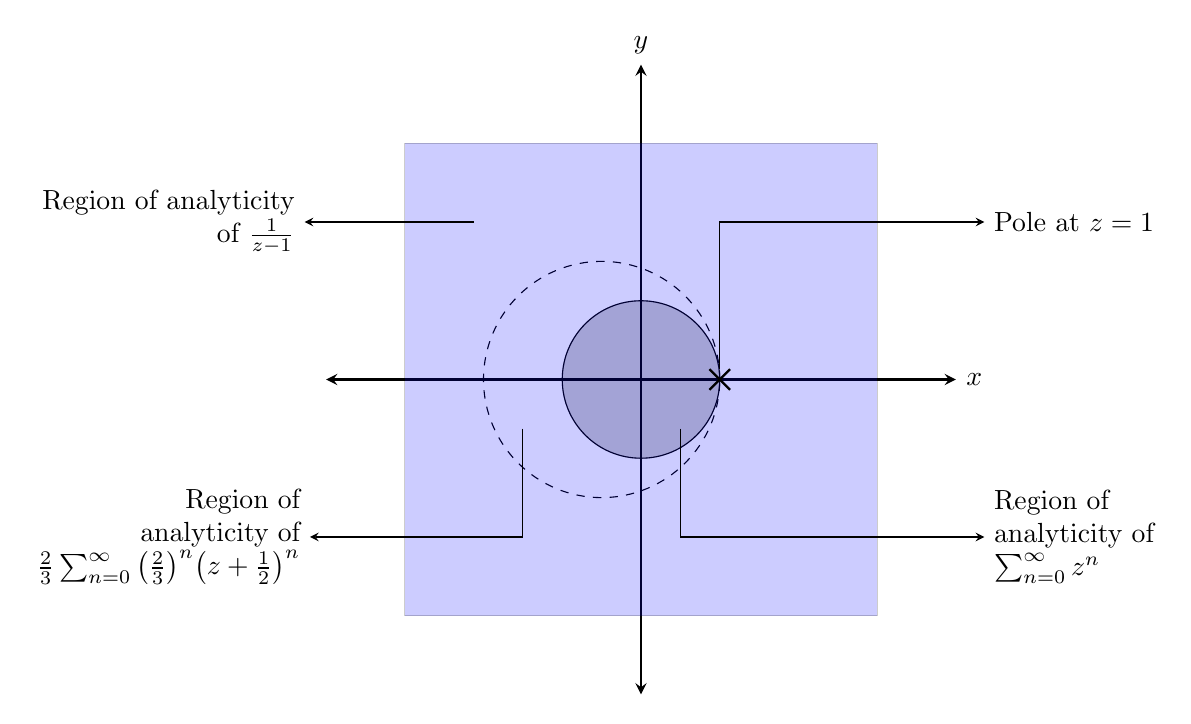
\begin{tikzpicture}
            \draw[thick,stealth-stealth] (-4,0)--(4,0) node[right] {$x$};
            \draw[thick,stealth-stealth] (0,-4)--(0,4) node[above] {$y$};
            \draw(0,0) circle (1);
            \draw[dashed](-0.5,0) circle (1.5);
            \draw[fill=black, opacity= 0.2](0,0) circle (1);
            \draw[fill=blue, opacity= 0.2](-3,-3)--(-3,3)--(3,3)--(3,-3)--cycle;
            
            \node (f11) at (-2,2) {};
            \node (f1) [align= right] at (-6,2) {Region of analyticity\\of $\frac{1}{z-1}$};
            \node (f22) at (0.5,-0.5) {};
            \node (f2) [align= left] at (5.5,-2) {Region of \\analyticity of\\ $\sum_{n=0}^{\infty}z^n$};
            \node (f33) at (-1.5,-0.5) {};
            \node (f3) [align= right] at (-6, -2) {Region of \\analyticity of \\$\frac{2}{3}\sum_{n=0}^{\infty}\qty(\frac{2}{3})^n\qty(z+\frac{1}{2})^n$};
            \draw[-stealth] (f11)--(f1);
            \draw[-stealth] (f22)|-(f2);
            \draw[-stealth] (f33)|-(f3);
            \node (p)[thick, cross out,draw] at (1,0) {};
            \node (p1) [align= left] at (5.5,2) {Pole at $z=1$};
            \draw[-stealth] (p)|-(p1);

        \end{tikzpicture} 
        \caption{\emph{Analytic continuation of $f(z)= \sum_{n=0}^{\infty}z^n$}}\label{analytic cont}        
    \end{center}
\end{figure}

\textbf{Analytic Continuation}: Say a function $f(z)$ is analytic in some region. Let's say we find another representation of the function which matches the original one point-by-point, but is analytic in some different region. There is an overlap region and if the second region is bigger than the first one then the second region is the analytic continuation of the same function. 

Say I want a power series at the point $z= -1/2$. I can then work backwards from $f(z)= \frac{1}{1-z}= \frac{1}{\frac{3}{2}- \qty(z+\frac{1}{2})}$. This can then be written as a binomial series: 
\[ \frac{1}{1-z}= \frac{2}{3}\qty[1-\frac{2}{3}\qty(z+\frac{1}{2})]^{-1}= \frac{2}{3}\sum_{n=0}^{\infty} \qty(\frac{2}{3})^n\qty(z+\frac{1}{2})^n
\]
This is the same function with an entirely different form of power series since it is expanded about the point $z=-1/2$. This series will clearly converge for $$\qty|\frac{2}{3}\qty(z+\frac{1}{2})|<1\Rightarrow \qty|z+\frac{1}{2}|<\frac{3}{2}$$
This is a circle centered at $-1/2$ with a radius of $1.5$. We can take any point within this circle, find another power series representation which is analytic within some other circle and continue doing this till we cover the entire complex plane. But all of these power series representations will have a singularity at $z=1$ since the \emph{master function} from where all these series come from has a singularity at $z=1$. 

\subsection{On the Circle of Convergence}

\emph{A given analytic function may have an infinite number of representations, each valid (analytic) in different regions. These representations are absolutely convergent inside the circle of convergence, divergent outside it, but no general statement can be made of what happens \emph{on} the circle of convergence.}

For example, $-1$ lies on the circle of convergence of $f(z)= \sum_{n=0}^{\infty} z^n$. But $z=-1$ gives $f(z)= 1-1+1-1+1-1\dots$. The series oscillates between $1$ and $0$. This can still be of some use. The average of the two partial sums is $1/2$. And surprisingly $\frac{1}{1-z}\big|_{z= -1/2}= 1/2$. Similarly, for $z=i, f(z)= 1+i-1-i+\dots$. The partial sums are $1, 1+i, i, 0$ and the average is $\frac{1+i}{2}= \frac{1-i^2}{2(1-i)}= \frac{1}{1-i}= \frac{1}{1-z}\big|_{z= i}$. This sort of sum is called the \emph{Cesaro Sum}. 

\textbf{On Cesaro Sums}: The arithmetic average of all the partial sums is equal to the value of the analytic continuation of that function at that point.

\textbf{On singularities}: The function which any power series represents must have at least one singularity on the circle of convergence. 

Anything can happen on the circle of convergence. A series can diverge, oscillate (as we saw), as well as absolutely converge. For example, the function $\sum_{n=1}^{\infty} \frac{z^n}{n^2}$ has a radius of convergence of: $$\lim_{n\to\infty}\qty|\frac{z^n (n+1)^2}{z^{n+1} n^2}|= \frac{1}{|z|}\Rightarrow |z|\leq 1$$
$R= 1$, and at $z= 1, \ f(z)= \sum_{n=1}^{\infty} \frac{1}{n^2}<\infty$. 

However, we said that every power series must have at least one singularity on the circle of convergence and the above function looks like it behaves regularly at all points on the circle! The singularity in this case is subtle, and it \emph{is} at $z= 1$. The subtlety can be seen using a function like $(z-1)\ln(z-1)$. At $z-1$, the log is undefined, and tends to infinity, whereas the $(z-1)$ term tends to $0$. The power term is stronger and thus the limit of this function at $z=1$ is $0$. The singular part of the function vanishes, however it is \emph{still} singular. 

As an example of more than one singularity, take the function $f(z)= z+ z^2 + z^4 + z^8\dots= \sum_{n=0}^{\infty} z^{2^n}$. The radius of convergence is $|z|<1$. But at $z=1$, the series obviously diverges, thus $z=1$ is a singularity. But since $f(z^2)= z^2+ z^4+ z^8+\dots$, then $f(z)$ can be rewritten as $f(z)= z+ f(z^2)$. Since $f(1)$ can be obtainted from $z=\pm 1$, we deduce that $f(z)$ has singularities at $\pm 1$. Again, we can again write $f(z)= z+ z^2 + f(z^4)$ which shows that $f(z)$ has singularities at $\pm 1$ and $\pm i$. Continuing, we find that the function has a lot of singularities on the unit circle. This barrier of singularities of $f(z)$ prevents it from having an analytic continuation outside $|z|<1$. The unit circle forms a \emph{natural boundary} for this function. These kinds of series are called \emph{lacunary series} from the fact that the successive powers of $z$ have large `gaps', or \emph{lacunas}. 

\end{document}